\documentclass[12pt,a4paper]{article}
\usepackage[utf8]{inputenc}
\usepackage[T1]{fontenc}
\usepackage{amsmath,amssymb}
\usepackage{pgfplots}
\usepackage{tikz}
\usepackage{lmodern}
\usepackage{graphicx}
\usepackage{hyperref}
\usepackage{listings}
\usepackage{xcolor}
\usepackage{enumitem}
\usepackage{fancyhdr}
\usepackage{lastpage}
\usepackage[left=2.5cm,right=2.5cm,top=2.5cm,bottom=2.5cm]{geometry}
\usepackage[table]{xcolor}
\usepackage{array}
\usepackage{hyperref}
\usepackage{nameref}

\pagestyle{fancy}
\fancyhf{}
\renewcommand{\headrulewidth}{0pt}
\rfoot{\thepage\ af \pageref{LastPage}}

\title{Forløbsplan}
\author{Anders S. Østergaard}
\date{\today}

\definecolor{codegreen}{rgb}{0,0.6,0}
\definecolor{codegray}{rgb}{0.5,0.5,0.5}
\definecolor{codepurple}{rgb}{0.58,0,0.82}
\definecolor{backcolour}{rgb}{0.95,0.95,0.92}
\definecolor{darkerlightblue}{rgb}{0.1, 0.3, 0.5}

\lstdefinestyle{mystyle}{
	backgroundcolor=\color{backcolour},   
	commentstyle=\color{codegreen},
	keywordstyle=\color{darkerlightblue},
	numberstyle=\tiny\color{codegray},
	stringstyle=\color{codepurple},
	basicstyle=\ttfamily\footnotesize,
	breakatwhitespace=false,         
	breaklines=true,                 
	captionpos=b,                    
	keepspaces=true,                 
	numbers=left,                    
	numbersep=5pt,                  
	showspaces=false,                
	showstringspaces=false,
	showtabs=false,                  
	tabsize=2
}
\lstset{style=mystyle}
\usepackage{matlab-prettifier}
\usepackage{listings}
\usepackage{color}

\definecolor{mygreen}{rgb}{0,0.6,0}
\definecolor{mygray}{rgb}{0.5,0.5,0.5}
\definecolor{mymauve}{rgb}{0.58,0,0.82}

\lstset{ 
	backgroundcolor=\color{white},   % choose the background color; you must add \usepackage{color} or \usepackage{xcolor}; should come as last argument
	basicstyle=\footnotesize,        % the size of the fonts that are used for the code
	breakatwhitespace=false,         % sets if automatic breaks should only happen at whitespace
	breaklines=true,                 % sets automatic line breaking
	captionpos=b,                    % sets the caption-position to bottom
	commentstyle=\color{mygreen},    % comment style
	deletekeywords={...},            % if you want to delete keywords from the given language
	escapeinside={\%*}{*)},          % if you want to add LaTeX within your code
	extendedchars=true,              % lets you use non-ASCII characters; for 8-bits encodings only, does not work with UTF-8
	firstnumber=1000,                % start line enumeration with line 1000
	frame=single,	                   % adds a frame around the code
	keepspaces=true,                 % keeps spaces in text, useful for keeping indentation of code (possibly needs columns=flexible)
	keywordstyle=\color{blue},       % keyword style
	language=Octave,                 % the language of the code
	morekeywords={*,...},            % if you want to add more keywords to the set
	%numbers=left,                    % where to put the line-numbers; possible values are (none, left, right)
	numbersep=5pt,                   % how far the line-numbers are from the code
	numberstyle=\tiny\color{mygray}, % the style that is used for the line-numbers
	rulecolor=\color{black},         % if not set, the frame-color may be changed on line-breaks within not-black text (e.g. comments (green here))
	showspaces=false,                % show spaces everywhere adding particular underscores; it overrides 'showstringspaces'
	showstringspaces=false,          % underline spaces within strings only
	showtabs=false,                  % show tabs within strings adding particular underscores
	stepnumber=2,                    % the step between two line-numbers. If it's 1, each line will be numbered
	stringstyle=\color{mymauve},     % string literal style
	tabsize=2,	                   % sets default tabsize to 2 spaces
	title=\lstname                   % show the filename of files included with \lstinputlisting; also try caption instead of title
}
\begin{document}
	\begin{titlepage}
	\centering
	\vspace*{6cm}
	{\Huge\bfseries SWROB2\par Exam\par}
	\vspace{2cm}
	Submitted by: \par 
	\begin{table}[!h]
		\centering
		\begin{tabular}{|l|l|l|}
			\hline
			Study nr  & Name 					   & Study line\\\hline
			202005180 & Nicolaj Meldgaard Pedersen & E\\\hline
			202105443 & Johannes Baagøe 		   & E\\\hline
			201270449 & Anders Sandø Østergaard    & EP\\\hline
			201905293 & Daniel F. Borch Olsen	   & E\\\hline
		\end{tabular}
	\end{table}
	\vspace{4cm}
	Århus Universitet \par
	\vfill
	\today
\end{titlepage}
\pagenumbering{arabic}
\thispagestyle{empty}
\begin{abstract}
	\textit{This report presents the design, implementation, and evaluation of an advanced robotic system integrated with the Robot Operating System (ROS). The project leverages ROS's dynamic capabilities alongside sophisticated algorithms to enhance robotic functionalities in motion control, motion planning, perception using camera algorithms, localization, and mapping. Utilizing MATLAB and a specific hardware setup, the system demonstrates significant improvements in task efficiency and obstacle management within a controlled experimental setup. The findings highlight the system’s robustness in real-time operations and its potential for adaptation in varied automation scenarios. This study not only showcases the successful application of ROS in complex robotic tasks but also sets a foundation for future advancements in robotic automation. The report concludes with an analysis of experimental results, discussing the system's performance against predefined objectives and suggesting areas for further research.}
\end{abstract}
\clearpage
\tableofcontents
\clearpage
	\clearpage
	\section{Exercise: Reactive navigation and path planning}
	
	\subsection{Objective}
	The goal is to understand and be using Probabilistic Roadmap (PRM) in combination with the turtlebot.
	
	\subsection{Connection to the TurtleBot3 from powershell}
	For making the connection to the turtlebot we are connecting to the WiFi 
	\begin{itemize}
		\item \textbf{ssid:} turtlebot
		\item \textbf{password:} turtlebot3
	\end{itemize}
	from powershell type:
	\begin{center}
		\textit{ssh ubuntu@192.168.72.251}, \textit{password: turtlebot}
	\end{center}
	\subsection{Starting ROS on turtlebot from powershell}
	from powershell type
	\begin{center}
		\textit{roscore}
	\end{center}
	\subsection{Connection to TurtleBot3 from Matlab}
	For setting the ros environment variable and setting the IP on the host (turtlebot):
	\begin{lstlisting}[style=Matlab-editor]
setenv('ROS_MASTER_URI','http://192.168.72.251:11311')\end{lstlisting}
	For setting the IP on the local machine 
	\begin{lstlisting}
setenv('ROS_IP','192.168.72.220')\end{lstlisting}
	The following command is closing existing connection to be ensure that when the user is connection the robot isn't connected to anyone else
	\begin{lstlisting}[style=Matlab-editor]
rosshutdown();\end{lstlisting}
	This command will be doing the initialization of the connection between ROS and Matlab
	\begin{lstlisting}[style=Matlab-editor]
rosinit('http://192.168.72.251:11311','NodeHost','192.168.72.220');\end{lstlisting} 
	\vspace{1cm}
	\noindent\textbf{Matlab script for init}
	\begin{lstlisting}[style=Matlab-editor]
setenv('ROS_MASTER_URI','http://192.168.72.251:11311')
setenv('ROS_IP','192.168.72.220')
rosshutdown();
rosinit('http://192.168.72.251:11311','NodeHost','192.168.72.220');\end{lstlisting}
	\clearpage
	\subsection{Probabilistic Roadmap Algorithm (PRM)}
	The Probabilistic Roadmap Algorithm (PRM) is a method developed for navigating relatively large maps. To start, we create the PRM object as follows:
	\begin{lstlisting}[style=Matlab-editor]
		prm = PRM(shannon)
	\end{lstlisting}
	Following the object creation, we initiate the planning process by specifying the number of points in the roadmap:
	\begin{lstlisting}[style=Matlab-editor]
		prm.plan('npoints', 150)
	\end{lstlisting}
	Through this process, 150 roadmap nodes are created. Each point is connected to its neighbor by a direct line path that does not intersect any obstacles, thereby constructing a network encompassing the entire map.
	\\\\
	We can visualize the points by typing
	\begin{lstlisting}
prm.plot()\end{lstlisting} 
	as we can see on the figure then there are dots and lines on our map, where the dots are representing the points and the lines are obstacle free-path between the points.
	\section{Road map in Shannon}
	\subsection{Overview of the Code}
	This code demonstrates a process for simulating and navigating a robot within a virtual environment using the Robot Operating System (ROS) and specific robotics algorithms. It encompasses several steps from creating an environmental map, defining obstacles, planning a route, and finally steering the robot to follow the route. Below is what occurs in each of the key sections:
	
	\subsection{Creating a Binary Occupancy Map}
	A binary occupancy map (\texttt{binaryOccupancyMap}) is created to represent an environment measuring 6 by 4 meters with a resolution of 10 cells per meter. This map is used to define areas accessible to the robot and those blocked by obstacles, initially set up without any obstructions.
	
	\subsection{Defining Walls and Obstacles}
	A numerical array (\texttt{walls}) matching the map's size is created to represent the locations of walls and obstacles. Values are set to 1 to indicate the presence of an obstacle in specific cells (e.g., walls around the edge and three 'tables' as obstacles in the environment). This information is transferred to the occupancy map, rendering these areas inaccessible to the robot.
	
	\subsection{Inflating the Map}
	The map is "inflated" by enlarging the obstacle sizes on the map to account for the robot's size. This ensures the robot does not attempt to navigate too close to an obstacle, thereby risking collision.
	
	\subsection{Creating a Probabilistic Roadmap (PRM)}
	A probabilistic roadmap method is utilized to generate a route for the robot. This involves creating a network of randomly generated points in free space, which are then connected with paths that avoid obstacles. The method uses 500 points to cover the map, attempting to find a feasible route from a start to an end position.
	
	\subsection{Navigating the Route}
	The route found using the PRM is employed along with a pure pursuit algorithm to steer the robot. Pure pursuit is a guidance algorithm that continually adjusts the robot's speed and direction to follow a route consisting of a series of waypoints. The algorithm adjusts the robot's linear and angular velocities based on the robot's current position and the desired route.
	
	\subsection{Position and Velocity Updates}
	The robot's position is continually updated using feedback from its sensors (in this case, position and orientation from a tf topic in ROS). Speed control commands are sent to the robot based on calculations from the pure pursuit controller, until the robot reaches its goal within a defined tolerance.
	
	\subsection{Visual Representations}
	Various visual representations of the environment, the robot's planned route, and eventually the actual path the robot attempts to follow are plotted throughout the code. This includes:
	\begin{itemize}
		\item The initial occupancy map before inflation.
		\item The occupancy map after inflation, showing how the "sizes" of obstacles have been increased.
		\item The probabilistic roadmap with the planned route.
		\item Updates on the robot's position and route adjustments as it follows the planned path.
	\end{itemize}
	These figures provide visual feedback on how the robot interacts with its environment, navigates around obstacles, and ultimately attempts to reach its goal.
	
	\begin{lstlisting}[style=Matlab-editor]
%% Create a binary occupancy Map
% Here we create a map that is 10x10 meters with 1 square per meter. 
map = binaryOccupancyMap(6,4,10)

%% Create a numeric array with matching size
walls = zeros(40,60);

% Left wall
walls(1:40,1) = 1;
% Right wall
walls(1:40,60) = 1;
% Top wall
walls(1,1:60) = 1;
% Bottom wall
walls(40,1:60) =1;

% Creating obstacles
%Table 1
walls(1:30, 10:20) = 1;

%Table 2
walls(35:40,27:60) = 1;

%Table 3
walls(7:27,40:60) = 1;

setOccupancy(map,[1,1],walls,'grid')
show(map)

%% Inflate the map to account for the size of the robot. 
% We are inflating the obstacles by the radius of the robot and the robot
% is 20cm so by 0.1m. 
inflate(map, 0.2);
show(map)

%% Creating a Proberlistic Roadmap
%Generating a probabilistic roadmap with 500 points
PRM = mobileRobotPRM(map,500);
show(PRM)

%% Adding a start and goal and calculating a path
%Defining start/end locations as measured IRL
startLocation = [0.5 3.5];
endLocation = [5.5 3.65];

%Generating the path using the points in the probabilistic road map
path = findpath(PRM,startLocation,endLocation);
show(PRM)

%% Implementing the purepersuit algorithm from last exercise
%Creating publishers and subscribers 
vel_pub = rospublisher('/cmd_vel');
ang_sub = rossubscriber('/imu');
pos_sub = rossubscriber('/tf');

%Reset the pos
reset_pub = rospublisher('/reset');
send(reset_pub,rosmessage(reset_pub));

%Setting the initial position of the robot (should be ~0,0 wince we reset
%the robot)
pos = update_pos(pos_sub)

%Defining the controller and all it's parameters
controller = controllerPurePursuit;
controller.DesiredLinearVelocity = 0.2;
controller.MaxAngularVelocity = 2;

%We found that the robot is relatively stable with a LookAheadDistance of 0.4
controller.LookaheadDistance = 0.4;

%The path is defined as the points found by the PRM
controller.Waypoints = path;

%defining the radius, endpoint and initializing distanceToGoal
goalRadius = 0.1;
robotGoal = path(end,:);
distanceToGoal = norm(pos - robotGoal)

while(distanceToGoal > goalRadius)   
	%We start the loop by updating the position of the robot
	robotCurrentPose = update_pos(pos_sub);
	
	% Compute the controller outputs, i.e., the inputs to the robot
	[v, w] = controller(robotCurrentPose);
	
	%Then we update the angular and linear velocities based on the
	%controller outputs.
	update_vel(v,w,vel_pub)
	
	%At last we check the distance to goal for whether we have reached the
	%end of the path.
	distanceToGoal = norm(robotCurrentPose(1:2) - path(end, :)')
end

function [output] = update_pos(pos_sub)
	%We start by getting the transform data from the tf topic
	receive(pos_sub,10);
	
	%the x and y data is = to the x and y of the tf topic
	pos.x = pos_sub.LatestMessage.Transforms.Transform.Translation.X;
	pos.y = pos_sub.LatestMessage.Transforms.Transform.Translation.Y;
	
	%We use the function quat2angle to transform the angle from quaternion to
	%yaw in radians
	quat.X = pos_sub.LatestMessage.Transforms.Transform.Rotation.X;
	quat.Y = pos_sub.LatestMessage.Transforms.Transform.Rotation.Y;
	quat.Z = pos_sub.LatestMessage.Transforms.Transform.Rotation.Z;
	quat.W = pos_sub.LatestMessage.Transforms.Transform.Rotation.W;
	
	[roll,pitch,yaw] = quat2angle([quat.X,quat.Y,quat.Z,quat.W]);
	
	pos.theta = yaw;
	
	%In the end we output the data and add the initial position of the robot to
	%x and y
	output = [pos.x+0.5; pos.y+3.5; pos.theta];
end


function [true] = update_vel(v,w,vel_pub)
	%Very simple function. We get a new linear and angular velocity from the
	%controller and output it to the cmd_vel topic.
	twistmsg = rosmessage(vel_pub);
	
	twistmsg.Angular.Z = w;
	twistmsg.Linear.X = v;
	
	send(vel_pub,twistmsg);
end\end{lstlisting}
	\noindent % Forhindrer indrykning af den første linje i dokumentet
	Following figures \nameref{fig:1}, \nameref{fig:2}, \nameref{fig:3} and \nameref{fig:4} was plottet in Matlab
	\begin{figure}[!h]
		\begin{minipage}{0.5\textwidth}
			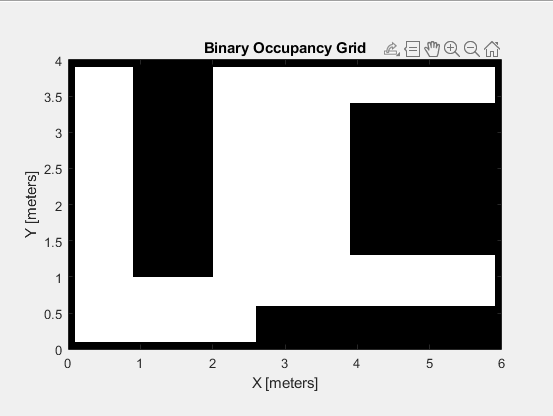
\includegraphics[width=\textwidth]{Binary Occupancy Map}
			\caption{Binary Occupancy Map}
			\label{fig:1}
		\end{minipage}%
		\begin{minipage}{0.5\textwidth}
			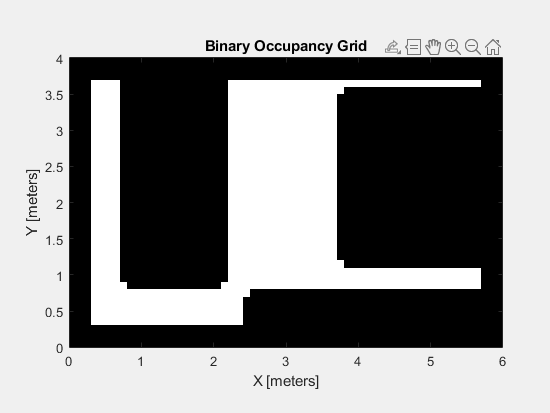
\includegraphics[width=\textwidth]{Inflated Binary Occupancy Map}
			\caption{Inflated Binary Occupancy Map}
			\label{fig:2}
		\end{minipage}
		
		\vspace{5mm} % Tilføjer vertikal plads mellem rækkerne
		
		\noindent
		\begin{minipage}{0.5\textwidth}
			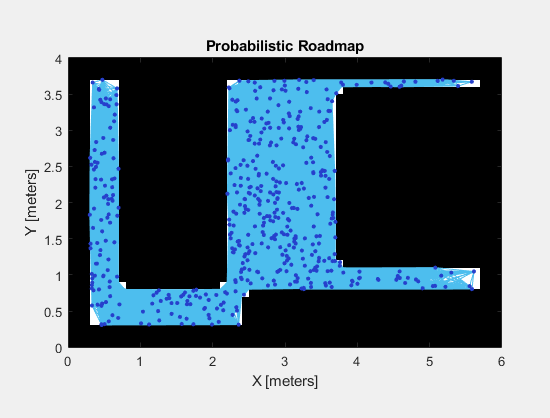
\includegraphics[width=\textwidth]{Proberlistic Roadmap}
			\caption{Proberlistic Roadmap}
			\label{fig:3}
		\end{minipage}%
		\begin{minipage}{0.5\textwidth}
			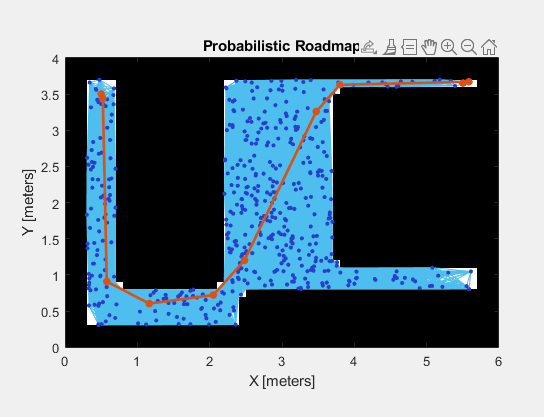
\includegraphics[width=\textwidth]{Proberlistic Roadmap with path}
			\caption{Proberlistic Roadmap with path}
			\label{fig:4}
		\end{minipage}
	\end{figure}
	
	
\end{document}